% Results section, included from report.tex. All tables are generated by
% scripts/make_report_tables.py from output/scenarios/scenario-results.json.

\subsubsection*{A. Service acceptance}

Table~\ref{tab:acc} and Figure~\ref{fig:acc} give hold-out acceptance for every
scenario. Updated FPPVS reaches the 70\% target in all six main scenarios. Its
mean acceptance ranges from \fppvsMinAcc\% (\fppvsWorstScenario) to
\fppvsMaxAcc\%, with an average of \fppvsMeanAcc\%. The lowest value in any single
seed was \fppvsLowestRun\%, so the target also holds run by run, not only on
average.

\begin{table}[H]
\centering\footnotesize
\setlength{\tabcolsep}{4pt}
\caption{Hold-out service acceptance (\%), mean $\pm$ standard deviation over
\numSeeds{} seeds. Best value per row in bold.}
\label{tab:acc}
\begin{tabular}{lccccc}
\toprule
Scenario (topology, load) & Updated (ours) & Original FPPVS & 2022 adaptation & Greedy & Random \\
\midrule
Backbone 0.5 & \textbf{99.6 $\pm$ 0.4} & 58.1 $\pm$ 4.1 & 68.1 $\pm$ 5.4 & 72.1 $\pm$ 5.8 & 73.2 $\pm$ 4.5 \\
Backbone 0.75 & \textbf{97.2 $\pm$ 2.1} & 50.1 $\pm$ 3.7 & 48.6 $\pm$ 15.3 & 62.6 $\pm$ 5.7 & 61.8 $\pm$ 3.8 \\
Backbone 1 & \textbf{86.4 $\pm$ 3.7} & 43.6 $\pm$ 5.1 & 44.5 $\pm$ 6.5 & 53.4 $\pm$ 5.1 & 55.3 $\pm$ 3.4 \\
Metro 0.5 & \textbf{99.0 $\pm$ 0.8} & 64.6 $\pm$ 10.2 & 74.0 $\pm$ 9.7 & 71.4 $\pm$ 3.0 & 72.1 $\pm$ 2.9 \\
Metro 0.75 & \textbf{93.0 $\pm$ 2.5} & 58.5 $\pm$ 6.6 & 59.1 $\pm$ 5.3 & 59.5 $\pm$ 2.9 & 59.9 $\pm$ 2.3 \\
Metro 1 & \textbf{81.3 $\pm$ 3.5} & 49.7 $\pm$ 4.5 & 49.4 $\pm$ 9.7 & 51.8 $\pm$ 3.6 & 52.6 $\pm$ 3.0 \\
\midrule \multicolumn{6}{l}{\emph{Overload stress tests (offered demand above total capacity)}} \\
Backbone 1.25 & \textbf{75.2 $\pm$ 2.9} & 38.7 $\pm$ 3.9 & 41.1 $\pm$ 3.0 & 49.3 $\pm$ 3.8 & 50.9 $\pm$ 2.7 \\
Backbone 1.5 & \textbf{65.2 $\pm$ 3.3} & 35.0 $\pm$ 4.2 & 38.4 $\pm$ 4.3 & 43.4 $\pm$ 4.1 & 44.2 $\pm$ 2.1 \\
Metro 1.25 & \textbf{69.2 $\pm$ 4.2} & 44.0 $\pm$ 2.9 & 40.5 $\pm$ 7.8 & 47.2 $\pm$ 2.1 & 46.9 $\pm$ 2.3 \\
Metro 1.5 & \textbf{60.6 $\pm$ 1.9} & 36.7 $\pm$ 5.0 & 42.2 $\pm$ 3.9 & 42.2 $\pm$ 2.7 & 43.1 $\pm$ 1.3 \\
\bottomrule
\end{tabular}
\end{table}

\begin{figure}[H]
\centering
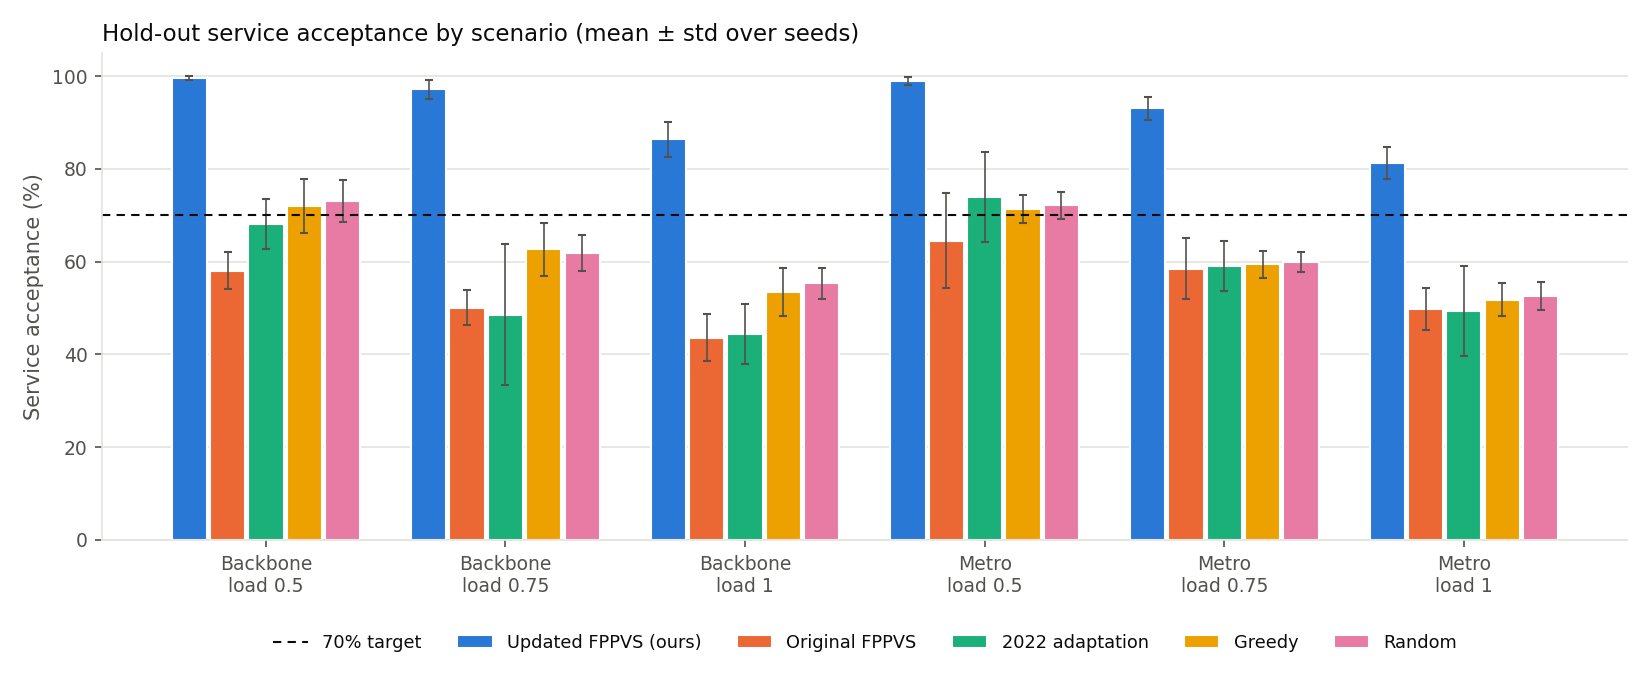
\includegraphics[width=\linewidth]{scenario-acceptance.png}
\caption{Hold-out acceptance per scenario. Error bars show one standard
deviation over seeds; the dashed line is the 70\% target.}
\label{fig:acc}
\end{figure}

\needspace{5\baselineskip}
\paragraph{Observations.}
\begin{itemize}
  \item Updated FPPVS is the best method in every scenario. At full load
  ($\rho=1$) it accepts 86.4\% on Backbone and 81.3\% on Metro.
  \item The original FPPVS reaches \origMinAcc--\origMaxAcc\% in the main
  scenarios (mean \origMeanAcc\%), and the 2022 adaptation reaches
  \zhangMinAcc--\zhangMaxAcc\% (mean \zhangMeanAcc\%). Updated FPPVS is
  \origGainMean{} points above the original and \zhangGainMean{} points above
  the 2022 adaptation on average.
  \item Both learning baselines often score below greedy and random. The
  reason is how infeasible choices are handled. Greedy and random run with our
  feasibility mask, so they never pick a DC that is already known to break
  bandwidth or latency. The original FPPVS and the 2022 adaptation check only
  compute while placing, as their methods describe, and find bandwidth and
  latency violations only when the whole chain is done (see Part E).
  \item The 2022 adaptation is the least stable method: its standard deviation
  across seeds reaches 15 points (Backbone, $\rho=0.75$). One reward value per
  episode (LTCR) gives the agent a weak learning signal.
  \item Greedy and random accept only 52--73\% even at light load. They spread
  VNFs over many DCs, so each request uses two to three times as much link
  bandwidth as updated FPPVS (Section~C), and links run out first.
  \item Metro is harder than Backbone at the same load. It has fewer DCs and
  fewer links, so there are fewer alternative paths when a link fills up.
\end{itemize}

\begin{figure}[H]
\centering
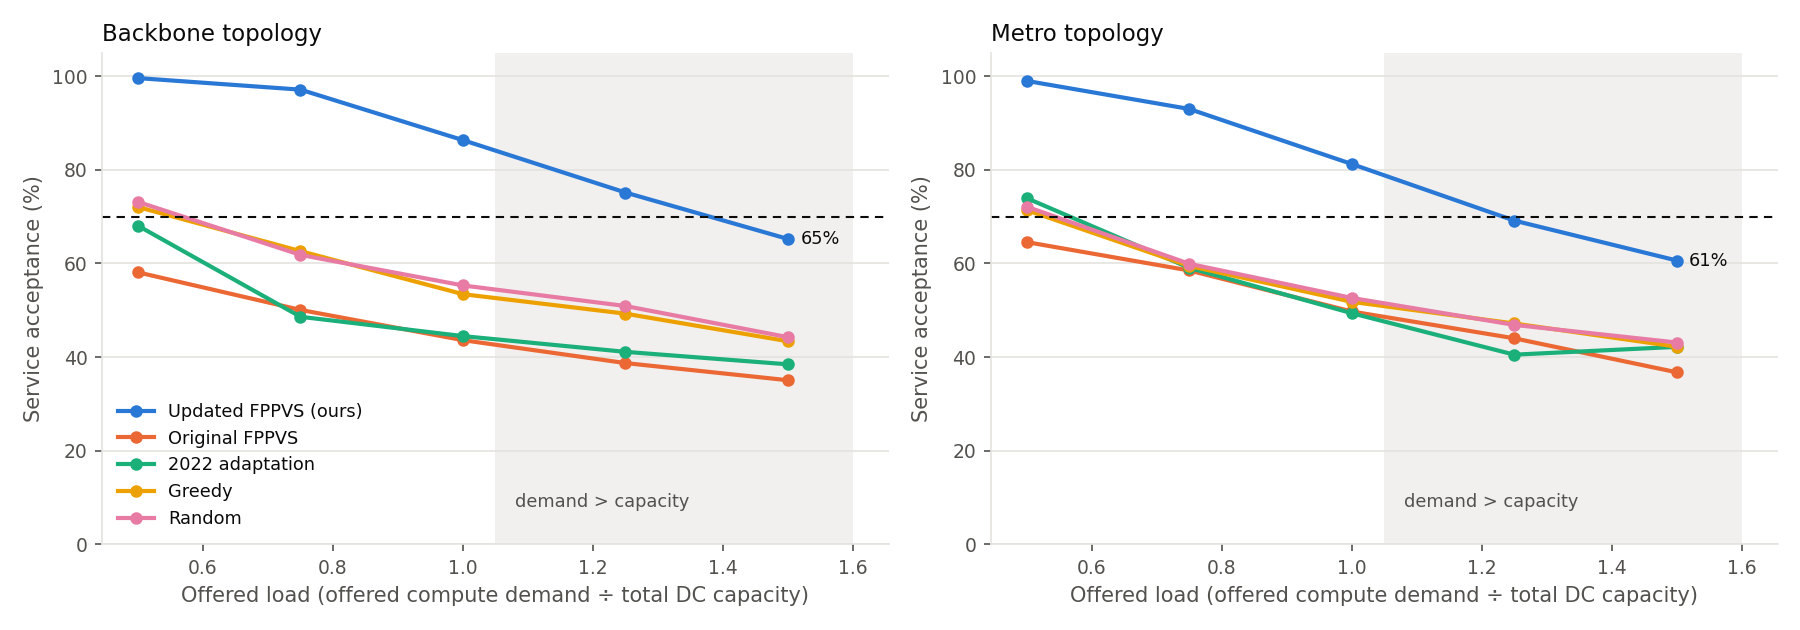
\includegraphics[width=\linewidth]{load-sweep.png}
\caption{Acceptance against offered load. The shaded area is overload, where the
average offered compute is larger than the total compute of the network.}
\label{fig:sweep}
\end{figure}

\paragraph{Overload.} Figure~\ref{fig:sweep} extends the load to 1.5 times the
network capacity. Updated FPPVS stays clearly ahead at every point: 75.2\%
(Backbone) and 69.2\% (Metro) at $\rho=1.25$, and 65.2\% and 60.6\% at
$\rho=1.5$. All other methods stay at or below 51\%. Below 70\% is unavoidable in
this region. At $\rho=1.5$ only about two thirds of the offered compute can fit
in the network at any time, whatever the placement policy. We therefore treat
these points as stress tests and not as part of the 70\% target.

\subsubsection*{B. Ablation study}

\begin{table}[H]
\centering\small
\caption{Ablation: hold-out acceptance (\%) of updated FPPVS with one part
switched off at a time.}
\label{tab:ablation}
\begin{tabular}{lcccccc}
\toprule
Scenario & Full & w/o sharing & w/o fairness & 1 agent & w/o retry & Prior only \\
\midrule
Backbone 0.5 & 99.6 $\pm$ 0.4 & 99.0 $\pm$ 1.0 & 99.4 $\pm$ 0.6 & 99.4 $\pm$ 0.6 & 99.5 $\pm$ 0.4 & 99.7 $\pm$ 0.3 \\
Backbone 0.75 & 97.2 $\pm$ 2.1 & 87.5 $\pm$ 3.0 & 97.0 $\pm$ 1.8 & 96.5 $\pm$ 2.2 & 96.7 $\pm$ 2.4 & 96.9 $\pm$ 2.2 \\
Backbone 1 & 86.4 $\pm$ 3.7 & 73.8 $\pm$ 3.1 & 85.6 $\pm$ 3.9 & 86.0 $\pm$ 3.4 & 85.4 $\pm$ 3.1 & 86.3 $\pm$ 2.8 \\
Metro 0.5 & 99.0 $\pm$ 0.8 & 97.9 $\pm$ 1.1 & 99.1 $\pm$ 1.0 & 98.5 $\pm$ 1.3 & 98.8 $\pm$ 0.9 & 99.0 $\pm$ 0.6 \\
Metro 0.75 & 93.0 $\pm$ 2.5 & 84.1 $\pm$ 2.3 & 93.4 $\pm$ 2.8 & 93.5 $\pm$ 3.2 & 93.5 $\pm$ 2.9 & 94.1 $\pm$ 2.2 \\
Metro 1 & 81.3 $\pm$ 3.5 & 70.6 $\pm$ 3.2 & 81.1 $\pm$ 2.9 & 81.0 $\pm$ 3.2 & 81.9 $\pm$ 4.0 & 81.7 $\pm$ 3.2 \\
\bottomrule
\end{tabular}
\end{table}

Table~\ref{tab:ablation} switches off one part of updated FPPVS at a time.
\begin{itemize}
  \item \textbf{VNF sharing matters most.} Without it, acceptance falls by 9--13
  points at $\rho\ge0.75$ (for example 86.4\% to 73.8\% on Backbone at
  $\rho=1$). Every VNF then pays its own instance overhead, so the DCs fill up
  sooner.
  \item \textbf{Fairness bonus, single vs.\ federated training and retries}
  change acceptance by about one point or less, which is within the
  seed-to-seed spread. Fairness is meant to balance throughput between flows, not
  to raise acceptance, so this is expected. Retries help only in the rare case
  where the first placement hits a dead end.
  \item \textbf{The learned network adds little over its prior.} ``Prior only''
  uses the same mask, prior and retries with no neural network, and it is within
  about one point of the full method everywhere. We report this openly: in our
  experiments the gains come mainly from the problem modifications (mask, sharing
  model, prior), not from the reinforcement learning itself. One reason is
  limitation L6: each episode covers only one request, so the agent sees little
  of the long-term effect of its choices.
\end{itemize}

\subsubsection*{C. Resource usage}

Figure~\ref{fig:res} and Table~\ref{tab:res} show the resources each method holds
for the services it runs. Table~\ref{tab:savings} summarises the difference
between updated FPPVS and each other method, averaged over the six main
scenarios.

\begin{figure}[H]
\centering
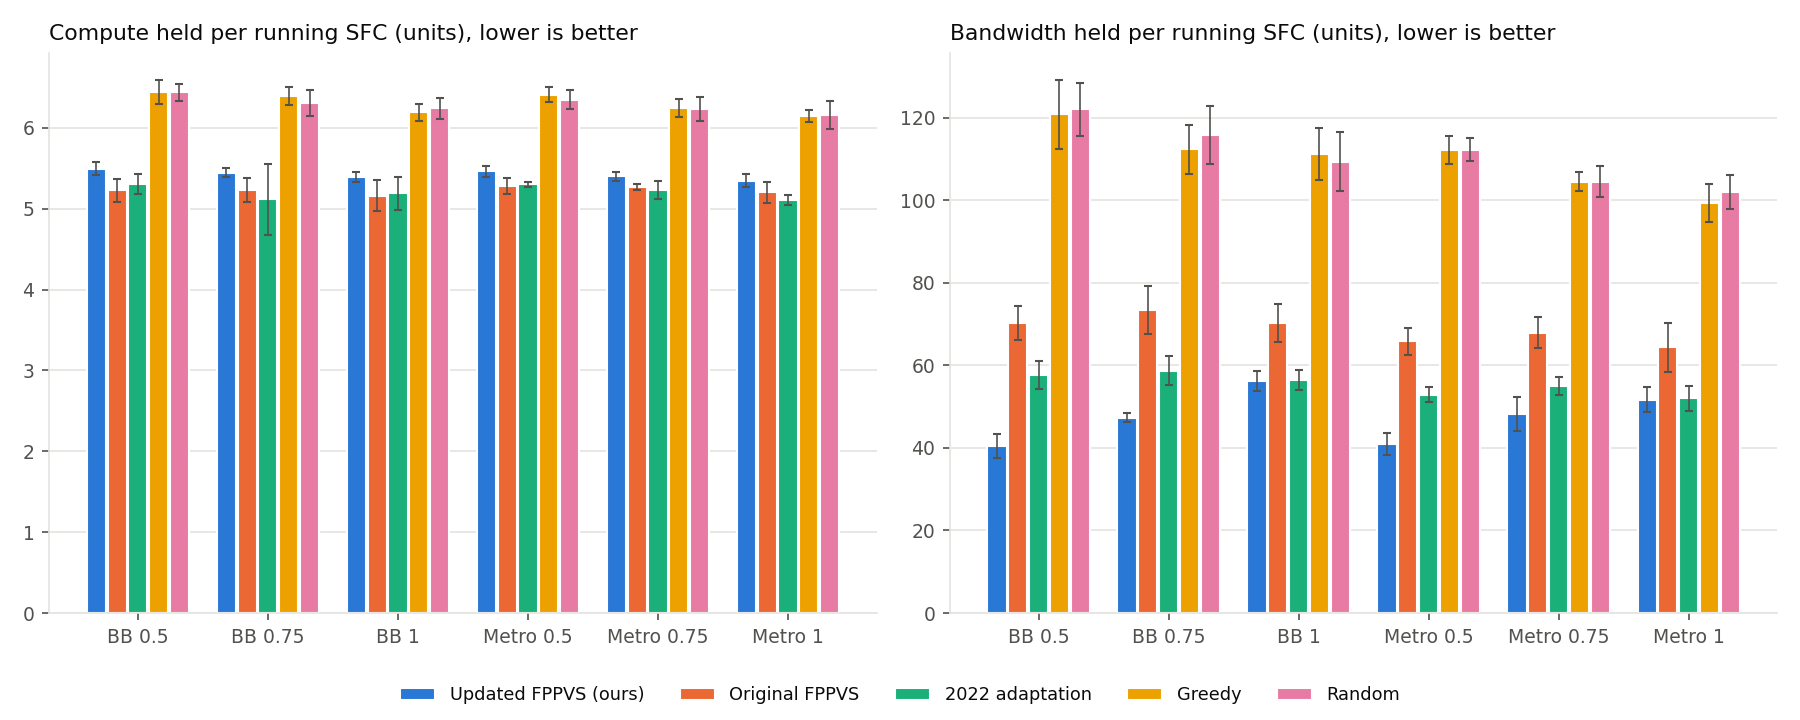
\includegraphics[width=\linewidth]{scenario-resources.png}
\caption{Compute (left) and bandwidth (right) held per running SFC, averaged over
time. Lower means each service costs less to keep running.}
\label{fig:res}
\end{figure}

\begin{table}[H]
\centering\small
\caption{Average reduction in resource use achieved by updated FPPVS over each
method (main scenarios; positive means updated FPPVS uses less, negative means
it uses more).}
\label{tab:savings}
\begin{tabular}{lcccc}
\toprule
Reduction vs. & Compute & Bandwidth & BW$\cdot$time & Instances \\
 & per SFC & per SFC & per accepted & per accepted \\
\midrule
Original FPPVS & -3.7\% & +30.7\% & +30.8\% & -6.5\% \\
2022 adaptation & -4.1\% & +14.2\% & +15.0\% & -8.3\% \\
Greedy & +14.0\% & +56.5\% & +57.1\% & +89.8\% \\
Random & +13.7\% & +56.9\% & +57.4\% & +89.8\% \\
\bottomrule
\end{tabular}
\end{table}

\begin{table}[H]
\centering\scriptsize
\setlength{\tabcolsep}{4pt}
\caption{Resource use and latency per scenario (mean over seeds; best per
column within a scenario in bold). ``Per acc.'' means per accepted SFC.}
\label{tab:res}
\begin{tabular}{llcccccc}
\toprule
Scenario & Method & Compute & Bandwidth & Compute$\cdot$time & BW$\cdot$time & Instances & Latency \\
 & & per SFC & per SFC & per acc. ($10^3$) & per acc. ($10^3$) & per acc. & (ms) \\
\midrule
Backbone 0.5 & Updated (ours) & 5.49 & \textbf{40.5} & 5.49 & \textbf{40.5} & 0.86 & \textbf{33.3} \\
 & Original FPPVS & \textbf{5.23} & 70.2 & \textbf{5.26} & 70.6 & 0.63 & 62.7 \\
 & 2022 adaptation & 5.31 & 57.6 & 5.35 & 58.0 & \textbf{0.60} & 64.7 \\
 & Greedy & 6.45 & 120.8 & 6.46 & 120.9 & 6.82 & 111.0 \\
 & Random & 6.44 & 122.0 & 6.53 & 123.7 & 6.77 & 111.6 \\
\midrule
Backbone 0.75 & Updated (ours) & 5.45 & \textbf{47.4} & 5.43 & \textbf{47.2} & 0.65 & \textbf{38.9} \\
 & Original FPPVS & 5.23 & 73.4 & 5.30 & 74.5 & \textbf{0.58} & 63.0 \\
 & 2022 adaptation & \textbf{5.11} & 58.7 & \textbf{5.19} & 59.8 & 0.62 & 68.1 \\
 & Greedy & 6.40 & 112.3 & 6.50 & 114.1 & 6.75 & 109.0 \\
 & Random & 6.31 & 115.9 & 6.38 & 117.3 & 6.64 & 109.8 \\
\midrule
Backbone 1 & Updated (ours) & 5.39 & \textbf{56.2} & 5.42 & \textbf{56.5} & \textbf{0.53} & \textbf{50.0} \\
 & Original FPPVS & \textbf{5.16} & 70.2 & \textbf{5.20} & 70.8 & 0.59 & 64.2 \\
 & 2022 adaptation & 5.19 & 56.5 & 5.28 & 57.4 & 0.61 & 67.2 \\
 & Greedy & 6.19 & 111.2 & 6.40 & 115.1 & 6.58 & 107.7 \\
 & Random & 6.24 & 109.4 & 6.27 & 110.1 & 6.58 & 108.1 \\
\midrule
Metro 0.5 & Updated (ours) & 5.46 & \textbf{41.0} & 5.57 & \textbf{41.9} & 0.85 & \textbf{33.7} \\
 & Original FPPVS & \textbf{5.28} & 65.8 & \textbf{5.31} & 66.3 & 0.70 & 56.7 \\
 & 2022 adaptation & 5.30 & 52.9 & 5.40 & 53.8 & \textbf{0.69} & 64.2 \\
 & Greedy & 6.41 & 112.2 & 6.44 & 112.7 & 6.76 & 109.2 \\
 & Random & 6.35 & 112.3 & 6.50 & 115.1 & 6.67 & 109.3 \\
\midrule
Metro 0.75 & Updated (ours) & 5.40 & \textbf{48.2} & 5.52 & \textbf{49.4} & 0.65 & \textbf{40.8} \\
 & Original FPPVS & 5.27 & 67.9 & 5.39 & 69.5 & 0.65 & 62.5 \\
 & 2022 adaptation & \textbf{5.23} & 55.0 & \textbf{5.32} & 55.9 & \textbf{0.63} & 67.4 \\
 & Greedy & 6.25 & 104.5 & 6.43 & 107.6 & 6.63 & 105.8 \\
 & Random & 6.23 & 104.5 & 6.52 & 109.5 & 6.61 & 107.2 \\
\midrule
Metro 1 & Updated (ours) & 5.35 & \textbf{51.6} & 5.44 & \textbf{52.5} & \textbf{0.55} & \textbf{48.6} \\
 & Original FPPVS & 5.21 & 64.3 & \textbf{5.28} & 65.4 & 0.67 & 62.2 \\
 & 2022 adaptation & \textbf{5.11} & 52.0 & 5.35 & 54.4 & 0.62 & 67.2 \\
 & Greedy & 6.15 & 99.4 & 6.46 & 104.4 & 6.53 & 104.1 \\
 & Random & 6.16 & 101.9 & 6.38 & 105.6 & 6.51 & 105.2 \\
\bottomrule
\end{tabular}
\end{table}

\needspace{5\baselineskip}
\paragraph{Observations.}
\begin{itemize}
  \item \textbf{Bandwidth.} Updated FPPVS holds the least bandwidth per running
  SFC in every main scenario: about 57\% less than greedy and random, 31\% less
  than the original FPPVS and 14\% less than the 2022 adaptation. Most of the
  saving comes from keeping consecutive VNFs on the same DC.
  \item \textbf{Compute and instances.} Against greedy and random, which do not
  share VNFs, updated FPPVS needs about 14\% less compute per service and about
  90\% fewer new instances (0.5--0.9 per accepted SFC instead of about 7).
  Against the original FPPVS and the 2022 adaptation, which both share VNFs, it
  uses about 4\% more compute per service and 7--8\% more instances per accepted
  request. Those two methods accept only about half of the requests, most likely
  the ones that were easy to fit, so their per-request averages come from an
  easier set. Even so, the difference is small next to the 35--39 points of
  extra acceptance.
  \item \textbf{Latency.} Mean latency of accepted requests is 33--50\,ms for
  updated FPPVS, 57--68\,ms for the original FPPVS and the 2022 adaptation,
  and 104--111\,ms for greedy and random. All are below the 100--150\,ms limits.
  The 2022 adaptation places the chain strictly in sequence (no parallel
  branches), so every monitor adds to the critical path.
  \item \textbf{Decision time.} Updated FPPVS needs 9--21\,ms per request,
  including the CNN forward pass and occasional retries. Greedy and random take
  about 3\,ms. Training one updated FPPVS model with 2000 episodes takes about
  \trainSeconds\,s on the CPU.
\end{itemize}

\subsubsection*{D. Effect of the algorithm alone}

Our main experiments use a different arrival process from our first version
(modification M1). To separate the effect of the algorithm from the effect of the
workload, we also ran the updated placement logic on the original workload: one
arrival per time unit, 100 requests, with almost nothing released during the run
(Table~\ref{tab:old}). The updated placement reaches 70.4\%, up from 10.4\% for
the original implementation. Acceptance is lower than in the Poisson runs mainly
because the original stream offers far more traffic than the network can hold.

\begin{table}[H]
\centering\small
\caption{Original workload (one arrival per time unit), 5 seeds. The upper
rows are from our first implementation; the lower rows use the updated
environment and placement logic.}
\label{tab:old}
\begin{tabular}{lc}
\toprule
Method (original workload, 100 requests) & Acceptance (\%) \\
\midrule
Original implementation, trained FDRL (5 seeds) & 10.4 $\pm$ 5.1 \\
Original implementation, greedy & 15.8 $\pm$ 3.1 \\
Original implementation, random & 11.6 $\pm$ 3.0 \\
\midrule
Updated FPPVS placement & 70.4 $\pm$ 2.9 \\
Greedy & 45.4 $\pm$ 2.1 \\
Random & 46.2 $\pm$ 2.2 \\
\bottomrule
\end{tabular}
\end{table}

\subsubsection*{E. Comparison with the original FPPVS and the 2022 adaptation}\label{sec:paper}

\paragraph{Same scenarios, same requests.} Table~\ref{tab:orig} puts the three
learning-based methods side by side. All three get 2000 training episodes and
are tested on the same hold-out requests.

\begin{table}[H]
\centering\small
\caption{Original FPPVS, the 2022 adaptation and updated FPPVS on identical
scenarios, mean over \numSeeds{} seeds. $^\ast$Gain = updated FPPVS minus the
better of the other two, in percentage points.}
\label{tab:orig}
\begin{tabular}{lccccccc}
\toprule
 & \multicolumn{4}{c}{Acceptance (\%)} & \multicolumn{3}{c}{Bandwidth per running SFC} \\
\cmidrule(lr){2-5}\cmidrule(lr){6-8}
Scenario & Original & 2022 & Updated & Gain$^\ast$ & Original & 2022 & Updated \\
\midrule
Backbone 0.5 & 58.1 & 68.1 & \textbf{99.6} & +31.6 & 70.2 & 57.6 & \textbf{40.5} \\
Backbone 0.75 & 50.1 & 48.6 & \textbf{97.2} & +47.1 & 73.4 & 58.7 & \textbf{47.4} \\
Backbone 1 & 43.6 & 44.5 & \textbf{86.4} & +41.9 & 70.2 & 56.5 & \textbf{56.2} \\
Metro 0.5 & 64.6 & 74.0 & \textbf{99.0} & +25.1 & 65.8 & 52.9 & \textbf{41.0} \\
Metro 0.75 & 58.5 & 59.1 & \textbf{93.0} & +34.0 & 67.9 & 55.0 & \textbf{48.2} \\
Metro 1 & 49.7 & 49.4 & \textbf{81.3} & +31.5 & 64.3 & 52.0 & \textbf{51.6} \\
\midrule \multicolumn{8}{l}{\emph{Overload stress tests}} \\
Backbone 1.25 & 38.7 & 41.1 & \textbf{75.2} & +34.1 & 68.2 & 57.1 & \textbf{59.9} \\
Backbone 1.5 & 35.0 & 38.4 & \textbf{65.2} & +26.8 & 67.7 & 57.8 & \textbf{59.5} \\
Metro 1.25 & 44.0 & 40.5 & \textbf{69.2} & +25.2 & 63.9 & 52.2 & \textbf{55.4} \\
Metro 1.5 & 36.7 & 42.2 & \textbf{60.6} & +18.5 & 62.4 & 51.7 & \textbf{55.9} \\
\bottomrule
\end{tabular}
\end{table}

\begin{itemize}
  \item Updated FPPVS accepts 25--47 percentage points more than the better of
  the two other learning methods in the main scenarios, and 18--34 points more
  under overload.
  \item Both other methods fail in the same way. For the original FPPVS, 80--86\%
  of rejections are link bandwidth and 14--19\% are latency violations; for the
  2022 adaptation the split is 65--71\% bandwidth and 28--35\% latency. Every one
  of these is found only after the whole chain has been placed, because both
  methods prune DCs by compute alone (limitation L3). The 2022 adaptation has more
  latency failures because it does not parallelize monitors.
  \item The original FPPVS's actor cannot tell DCs apart after global pooling
  (L5), so it tends to spread a chain over several DCs and uses the most
  bandwidth of the three. The 2022 adaptation's fully connected network keeps
  each DC in a fixed input position and uses less bandwidth than the original,
  but it still has no way to see bandwidth or latency before the chain is done.
\end{itemize}

\paragraph{Published numbers.} Table~\ref{tab:paper} shows the results published
in the FPPVS paper next to our three runs at full load.

\begin{table}[H]
\centering\small
\caption{Published FPPVS results (Tables 6 and 7 of the paper) next to our runs
of the original FPPVS, the 2022 adaptation and updated FPPVS at load 1.0. Values
come from different data and settings; see the text before comparing them.}
\label{tab:paper}
\begin{tabular}{llcccc}
\toprule
 & & Published & \multicolumn{3}{c}{Our runs, load 1.0} \\
\cmidrule(lr){4-6}
Topology & Metric & FPPVS (paper) & Original & 2022 & Updated \\
\midrule
Backbone & Acceptance (\%) & 88.1 & 43.6 & 44.5 & 86.4 \\
 & Latency (ms) & 134.4 & 64.2 & 67.2 & 50.0 \\
 & Resource utilization (\%) & 75.35 & 40.2 & 42.3 & 82.8 \\
\midrule
Metro & Acceptance (\%) & 75.9 & 49.7 & 49.4 & 81.3 \\
 & Latency (ms) & 160.1 & 62.2 & 67.2 & 48.6 \\
 & Resource utilization (\%) & 72.36 & 49.3 & 49.4 & 82.5 \\
\bottomrule
\end{tabular}
\end{table}

Our run of the original specification reaches 43.6\% (Backbone) and 49.7\%
(Metro), far below the 88.1\% and 75.9\% the paper reports. We could not
reproduce the published numbers, and we see four likely reasons:
\begin{enumerate}
  \item \textbf{Workload.} The paper's arrival rate is not given (L1). Its
  numbers may correspond to a lighter load than our $\rho=1$.
  \item \textbf{Data.} The paper uses the real USAnet and Italian operator
  topologies and traces (L2); we use random graphs of the same size.
  \item \textbf{Training budget.} The paper trains for 2000 iterations of 10
  episodes with 20 SFCs each, about 400{,}000 SFC placements. Our models see
  2000 episodes (one SFC each) on a laptop CPU.
  \item \textbf{Unstated details.} Several parts of the original method are not
  fully described (sharing capacity, exact state encoding, final-reward scale),
  so our reading of them may differ from the authors' code.
\end{enumerate}
Latency and utilization are also defined differently. Our latency counts link
delay and VNF processing on the critical path, and the paper's values (above
100\,ms) suggest it includes more delay components. Our utilization is the
time-averaged share of total compute in use. These rows indicate trends only.

What the comparison does show is consistent: under the same conditions, updated
FPPVS raises mean acceptance in the main scenarios from \origMeanAcc\% (original
FPPVS) and \zhangMeanAcc\% (2022 adaptation) to \fppvsMeanAcc\%. At full load,
updated FPPVS (86.4\% and 81.3\%) is in the same range as the paper's published
values, and it holds less bandwidth per running service than every other method.
